\chapter{Theoretical Background}
\label{theoretical_background}
 
This chapter will discuss the theoretical background knowledge that was part of the decision-making during the development process.
 
\section{Numerical Mathematics}
The science of the numerical mathematics is a branch of mathematics that concentrates on the research of solving continuous problems with discrete systems, such as a computer.
One of the main issues in numerical mathematics is the representation of fractional numbers. This is because computers can only represent a finite subset of decimals, due to memory and processing limitations.
This can lead to rounding errors that can have a significant impact on the precision of any calculation with fractional numbers.
Further, calculations with numbers that have a large amount of decimal places, require more calculation steps by the processor and therefore slow down the computation.\cite{quarteroni2007numerical}
 
\subsection{Floating-Point Arithmetic}
One way to represent fractional number is the floating point number system. With this system, numbers are stored in memory in two parts: the significant and its base. The significant represents the number as an integer, without the decimal point.
The base ($10^x$) describes the position of the decimal point in the original number.\cite{quarteroni2007numerical}
 
\subsection{Fixed-Point Arithmetic}
The fixed point representation of numbers on a numerical system, defines the fractional number with a fixed amount of rational numbers. Further, the amount of significant numbers and decimal places is fixed.
The intention behind this number representation is to simplify and therefore speed up numerical calculations.\cite{quarteroni2007numerical}
 
\section{Manufacturing Methods}
Nowadays, engineers have a broad spectrum of different manufacturing methods available when it comes to producing a part.
The decision which to choose should incorporate component specific properties such as the desired amount to be produced,
the general shape and material of the part, as well as the environment the part will be used in.
 
\subsection{Additive Manufacturing}
Additive manufacturing (AM) is a process, where material is build up in order to create the desired shape. AM has first appeared in 1981, with the first commercial available machine in 1988.
Additive manufacturing incorporates a wide variety of different manufacturing methods. The most well know Additive manufacturing method today probably is Fused Deposition Modeling (FDM), also known as 3D-Printing.
With FDM, a thin thermoplastic filament is molten in a "Print head" and then squeezed through a nozzle. The molten plastic is then laid down in layers onto a print bed, in order to create a 3D shape. This process is shown in Figure \ref{TheoPrinter}.
The core advantages of FDM are its speed and flexibility. This makes prototyping and small production batches very cost-effective and easy.
Further, because 3D-Printing is a layer by layer process, almost any shape can be created, this is especially important for shapes with undercuts and included geometry's.\cite{FraunhoferInstitutAM}
 
\begin{figure}
    \begin{center}
    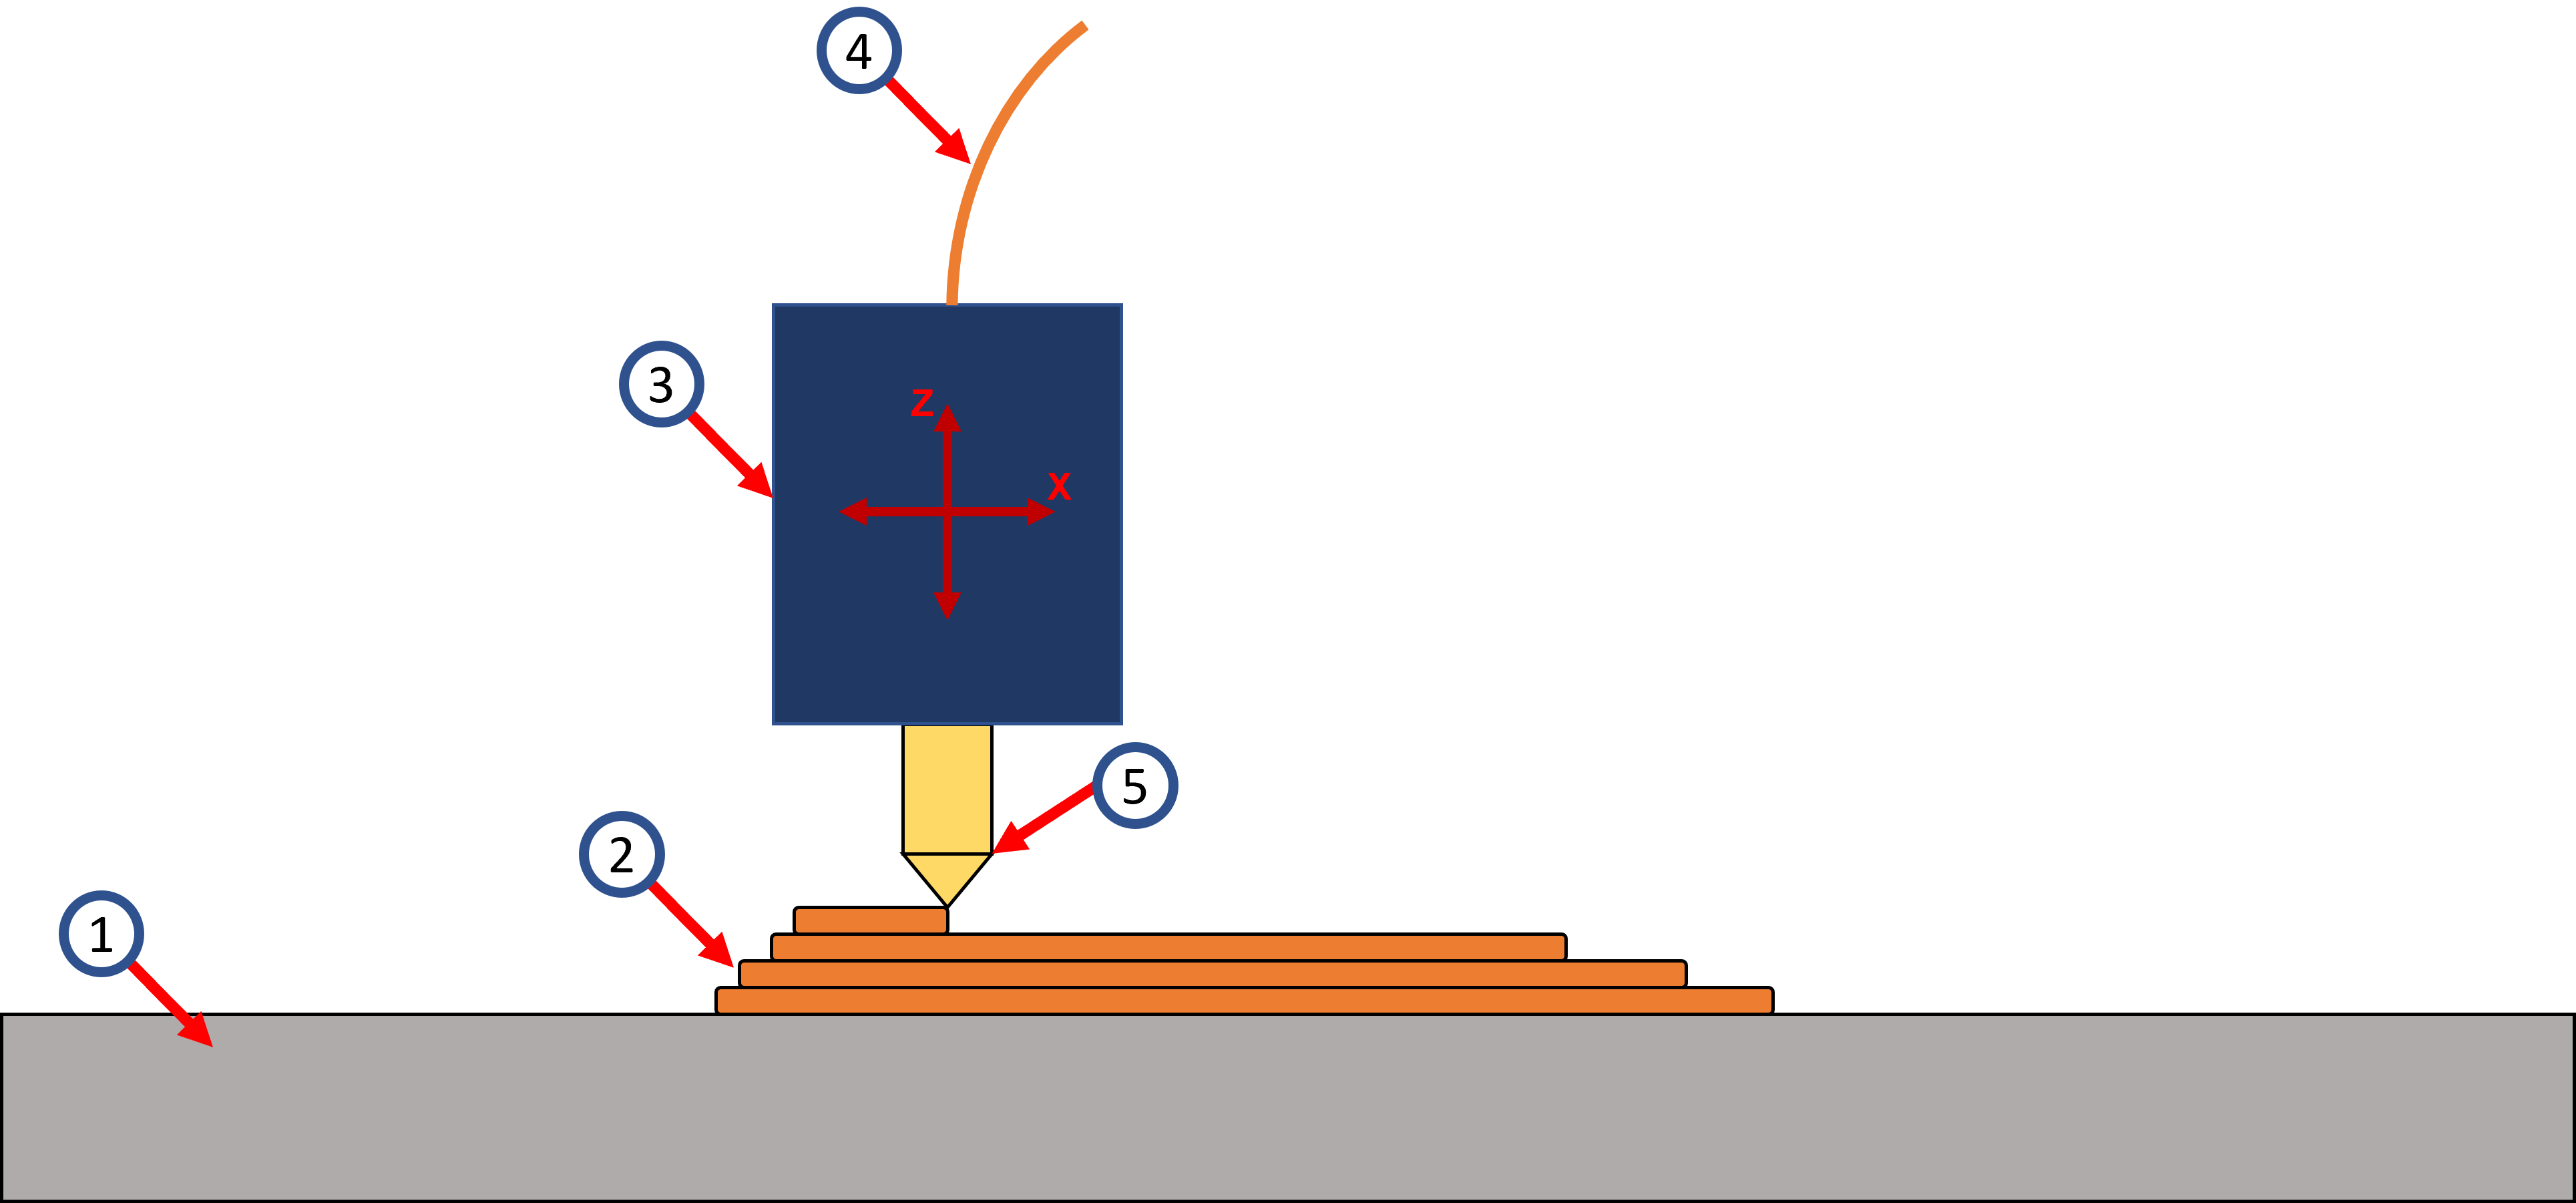
\includegraphics[width=12cm]{Pictures/TheoPrinter.png}
    \caption[2D Drawing of the 3D-Printing Process]{2D Drawing of the 3D-Printing Process; 1 - Print bed, 2 - Plastic layers, 3 - Print head, 4 - Plastic filament, 5 - Nozzle}
    \label{TheoPrinter}
    \end{center}
\end{figure}
 
\subsection{Subtractive Manufacturing}
Subtractive manufacturing is a process, where material is removed from a stock material in order to create a 2D or 3D shape. Two of the most common subtractive manufacturing processes are turning and milling.\\
Turning is a process where the stock material is rotated in a lathe and cut with a non-rotating tool. The tool itself only moves in X and Z direction. This process is shown in Figure \ref{TheoLathe}. For this reason, turning is especially well suited for the production of round parts.
 
\begin{figure}
    \begin{center}
    \includegraphics[width=12cm]{Pictures/Lathe.png}
    \caption[Picture of a turning process]{Picture of a turning process; 1 - Rotating work pice, 2 - Cutting tool, X - X Axis, Z - Z axis}
    \label{TheoLathe}
    \end{center}
\end{figure}
 
 
 
 
 

